\documentclass{article}
\usepackage[paperheight=13.5cm,paperwidth=16cm,margin=0cm]{geometry}
\usepackage{tikz}

\begin{document}

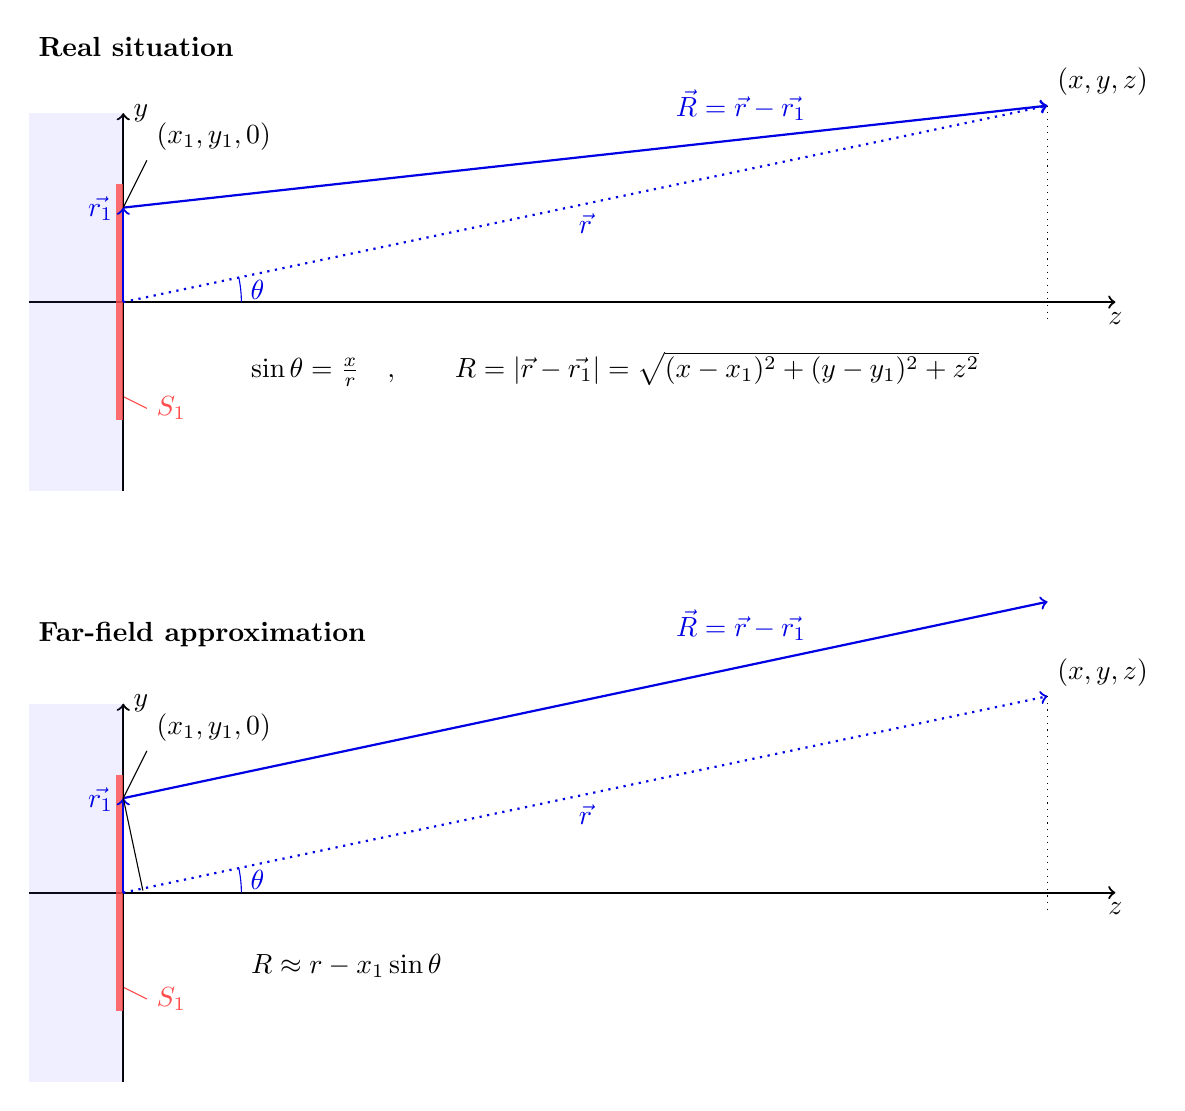
\begin{tikzpicture}[scale=3]%[>=stealth]

	\def\ymin{-0.8}
	\def\ymax{0.8}
	\def\zmin{-0.4}
	\def\zmax{4.2}
	
	\def\r{4.0}
	\def\ztext{0.5}
	
	\def\y1{0.4}
	\def\ya{0.5}
	\def\za{0.03}

    \def\angle{12}
	
	\def\yoff{-2.5}	
	
	% Colours
	\colorlet{wallcolor}{blue!60!white}
	\colorlet{aperturecolor}{red!70!white}
	\colorlet{pathcolor}{blue!90!black}
	
	% Styles  
	\tikzstyle{axisline}=[->, thick] 
	\tikzstyle{Rline} = [pathcolor, ->, thick]
	\tikzstyle{rline} = [pathcolor, ->, thick, dotted] 
	
	
	%== Real situation =======================================================
	\node[anchor=south west] at (\zmin, \ymax+0.2) {\textbf{Real situation}};

	\node[anchor=south west] at (\ztext, -0.4) 
			{$\sin \theta =\frac{x}{r} \quad,\qquad R= |\vec{r}-\vec{r_1}| = \sqrt{(x-x_1)^2 + (y-y_1)^2 +z^2}$}
			coordinate (textpos);
	
	\draw[aperturecolor](0, -\y1) -- ++(0.10, -0.05)
		node[aperturecolor, anchor=west] {$S_1$};

	% Axes
	\draw[axisline] (\zmin, 0) -- (\zmax, 0)  node(zaxis)[below]{$z$};
	\draw[axisline] (0, \ymin) -- (0, \ymax)  node(yaxis)[right]{$y$};
	
	% Wall
	\fill[fill=wallcolor, opacity=0.1] (\zmin, \ymin) rectangle  (0.0, \ymax);
	\fill[fill=aperturecolor, opacity=0.8] (-\za, -\ya) rectangle (0.0, \ya);
	
	% Sound paths
	\draw[rline] (0, 0) -- ++(\angle:\r)  
				node[midway, anchor=north]{$\vec{r}$}
				coordinate (xf);

	\draw[Rline] (0, \y1) -- (xf)
				node[near end, anchor=south east]{$\vec{R} = \vec{r} - \vec{r_1}$};

	\draw[pathcolor, ->, thick] (0, 0) -- (0, \y1) 
				node[near end, anchor=south east]{$\vec{r_1}$};
				
	\draw[pathcolor] (0.5, 0.0)  arc(0:\angle:0.5) node[midway, right, pathcolor] {$\theta$};

	\draw[dotted] (xf) -- (xf |- zaxis);
	\node[anchor=south west] at (xf)  {$(x,y,z)$};
	\draw(0, \y1) -- ++(0.10, 0.20) node [anchor=south west] {$(x_1,y_1,0)$};
	
	%== Far-field aproximation ===================================================
	\node[anchor=south west] at (\zmin, \ymax+0.2+\yoff) {\textbf{Far-field approximation}};

	\node[anchor=south west] at (\ztext, -0.4+\yoff) 
		{$R \approx r - x_1 \sin \theta$};
	
	\draw[aperturecolor](0, -\y1+\yoff) -- ++(0.10, -0.05)
		node[aperturecolor, anchor=west] {$S_1$};

	% Axes
	\draw[axisline] (\zmin, \yoff) -- (\zmax, \yoff)  node(zaxis)[below]{$z$};
	\draw[axisline] (0, \ymin+\yoff) -- (0, \ymax+\yoff)  node(yaxis)[right]{$y$};
	
	% Wall
	\fill[fill=wallcolor, opacity=0.1] (\zmin, \ymin+\yoff) rectangle  (0.0, \ymax+\yoff);
	\fill[fill=aperturecolor, opacity=0.8] (-\za, -\ya+\yoff) rectangle (0.0, \ya+\yoff);
	
	% Sound paths
	\draw[rline] (0, \yoff) -- ++(\angle:\r)  
				node(rline)[midway, anchor=north]{$\vec{r}$}
				coordinate (xf);
				
	\draw[Rline] (0, \y1+\yoff) -- ++(\angle:\r)  
				node[near end, anchor=south east]{$\vec{R} = \vec{r} - \vec{r_1}$};

	\draw[pathcolor] (0.5, +\yoff)  arc(0:\angle:0.5) node[midway, right, pathcolor] {$\theta$};

	\draw[pathcolor, ->, thick] (0, \yoff) -- (0, \y1+\yoff) coordinate (r1)
			node[near end, anchor=south east]{$\vec{r_1}$};
			
	\draw[color=black, -] (r1) -- ++(-90+\angle:\y1);

	\draw[dotted] (xf) -- (xf |- zaxis);
	\node[anchor=south west] at (xf)  {$(x,y,z)$};
	
	\draw(0, \y1+\yoff) -- ++(0.10, 0.20) node [anchor=south west] {$(x_1,y_1,0)$};


\end{tikzpicture}

\end{document}
